%%%%%%%%%%%%%%%%%%%%%%%%%%%%%%%%%%%%%%%%%%%%%%%%%%%%%%%%%%%%%%%%%%%%%
% LaTeX Template: Project Titlepage Modified (v 0.1) by rcx
%
% Original Source: http://www.howtotex.com
% Date: February 2014
% 
% This is a title page template which be used for articles & reports.
% 
% This is the modified version of the original Latex template from
% aforementioned website.
% 
%%%%%%%%%%%%%%%%%%%%%%%%%%%%%%%%%%%%%%%%%%%%%%%%%%%%%%%%%%%%%%%%%%%%%%

\documentclass[12pt]{article}
\usepackage[a4paper]{geometry}
\usepackage[myheadings]{fullpage}
\usepackage{fancyhdr}
\usepackage{lastpage}
\usepackage{graphicx, wrapfig, subcaption, setspace, booktabs}
\usepackage[T1]{fontenc}
\usepackage[font=small, labelfont=bf]{caption}
\usepackage{fourier}
\usepackage[protrusion=true, expansion=true]{microtype}
\usepackage[english]{babel}
\usepackage{sectsty}
\usepackage{url, lipsum}
\usepackage{multirow}
\usepackage{listings}

\usepackage{lmodern}  % for bold teletype font
\usepackage{amsmath}  % for \hookrightarrow
\usepackage{xcolor}   % for \textcolor

\lstset{
  basicstyle=\ttfamily,
  columns=fullflexible,
  frame=single,
  breaklines=true,
  postbreak=\mbox{\textcolor{red}{$\hookrightarrow$}\space},
}


\newcommand{\HRule}[1]{\rule{\linewidth}{#1}}
\onehalfspacing
\setcounter{tocdepth}{5}
\setcounter{secnumdepth}{5}

% Get the month and the year
\usepackage{datetime}
\newdateformat{monthyeardate}{
  \monthname[\THEMONTH], \THEYEAR
  }

%-------------------------------------------------------------------------------
% HEADER & FOOTER
%-------------------------------------------------------------------------------
\pagestyle{fancy}
\fancyhf{}
\setlength\headheight{15pt}
\fancyhead[L]{40274024}
\fancyhead[R]{Edinburgh Napier University}
\fancyfoot[R]{Page \thepage\ of \pageref{LastPage}}
%-------------------------------------------------------------------------------
% TITLE PAGE
%-------------------------------------------------------------------------------

\begin{document}

\title{ \normalsize \textsc{SET09120 Data Analytics}
		\\ [2.0cm]
		\HRule{0.5pt} \\
		\LARGE \textbf{\uppercase{Data Mining}}
		\HRule{2pt} \\ [0.5cm]
		\normalsize \monthyeardate\today \vspace*{5\baselineskip}}

\author{
		40274024 \\ 
		Edinburgh Napier University \\
		School of Computing 
		\date{}}

\maketitle

\newpage

%-------------------------------------------------------------------------------
% Section title formatting
\sectionfont{\scshape}
%-------------------------------------------------------------------------------

%-------------------------------------------------------------------------------
% BODY
%-------------------------------------------------------------------------------

\section{Introduction}
The aim of this coursework was to prepare and analyse a given dataset using machine learning and data mining. A variety of different algorithms were used that covered classification, clustering, association and regression. The data was analysed for relationships and patterns and a set of rules were produced per algorithms in order to better define these. OpenRefine was used to prepare and clean the data. Two ARFF files were created, a full dataset with numeric and nominal values a nominal only dataset. Weka was used for the machine learning analysis.

%-------------------------------------------------------------------------------
% Cleaning
%-------------------------------------------------------------------------------

\section{Data Preparation}
\subsection{Data cleaning}
OpenRefine was used in order to clean the provided dataset and allow it to be exported in an error free format for analysis.
Some values in the data had to be changed in order to fix any errors, such as typos.

\begin{table}[h!]
\centering
\begin{tabular}{|c|c|c|}
\hline
\multicolumn{1}{|l|}{Error Column} & Error Type & \multicolumn{1}{r|}{Qty of Errors} \\ \hline
purpose & Spelling errors & 4 \\
credit\_amount & Out of range numbers & 7 \\
age & typos, numbers out of range & 4 \\
job & typos, invalid values & 1 \\ \hline
\end{tabular}
\caption{Data Cleaning errors}
\label{fig:data_cleaning}
\end{table}

Typos were corrected to bring them in line with the same style as the rest of the data and capital letters were removed. Erratic values were corrected by inferring an average value based on trends within the data. Other attributes were also taken into consideration when inferring values such as the reason for the loan, age and employment status. Detailed data corrections can be seen in Table~\ref{fig:error_corrections}.

\begin{table}
\centering
\begin{tabular}{|c|c|c|}
\hline
Column & Incorrect data & Correction \\ \hline
\multirow{8}{*}{credit\_amount} & 111328000 & 8582 (inferred from data) \\
 & 13580000 & 8582 (inferred from data) \\
 & 63610000 & 6361 \\
 & 19280000 & 1928 \\
 & 13860000 & 1386 \\
 & 5180000 & 518 \\
 & 5850000 & 585 \\
 & 7190000 & 7190 \\ \hline
\multirow{4}{*}{age} & - values & removed - \\
 & decimal values & removed decimal and mantissa \\
 & 1 & 19 (inferred from data) \\
 & 222 & 22 (input error) \\
 & 333 & 33 (input error) \\
 & 6 & 26 (inferred from data) \\ \hline
job & yes & skilled (inferred from data) \\ \hline
\end{tabular}
\caption{Error corrections}
\label{fig:error_corrections}
\end{table}

A second copy of the cleaned data was produced with the numeric values converted to nominal values to allow associate algorithms such as Apriori to be used.

\subsection{Data conversion}
The dataset that was provided was given in Micorosoft's XLSX format, this had to be converted to an Attribute-Relation File Format (ARFF) in order to be processed by Weka. OpenRefine accepts XLSX format so this was used at the data cleaning stage then outputted to a comma separated value file (csv). Weka contains a built in tool, called ARFF viewer, that converts csv files to ARFF. The case number column was left in the data however the column was removed in Weka to allow appropriate rules to be created.
%-------------------------------------------------------------------------------
% Analysis
%-------------------------------------------------------------------------------
\section{Data Analytics}
\subsection{Classification}
% talk about accuracy and confusion matrix a= good b= bad 
% pruning

\begin{lstlisting}[caption="J48 configuration"\label{fig:j48_config}]
J48 -C 0.25 -M 2
\end{lstlisting}

The cleaned dataset was analysed using the J48 classification algorithm. J48 was chosen as it outputs decision trees that can easily be visualised and rules can be drawn from it. The algorithm was run on the job attribute with the setting shown in Listing~\ref{fig:j48_config}. In order to produce a usable tree the 'case\_no', 'checking\_status', 'personal\_status' and 'class' attributes were excluded from the tree. The algorithm produced a pruned tree with 18 nodes and 15 leaves, the resulting rules that can be seen from the tree are shown in Listing~\ref{fig:j48_rules}. The model produced accurately classifies 65.5\% of cases, this is relatively low and can also be seen in the confusion matrix (Figure:~\ref{fig:j48_conf_matrix}). The confusion matrix shows that only 6 cases of A were incorrectly classified where as all 200 cases of B (unskilled resident) were incorrectly classified. In C (high qualif/self emp/mgmt) it can be seen that 31 cases out of 148 were correctly classified by this model and lastly in D (unemp/unskilled non res) nothing was correctly classified. These large margins of error, especially B, are the reason for the low overall accuracy of the model however some general rules can still be created. The low overall score of this model also, in turn, brings down the accuracy of the rules.

\begin{figure}
    \centering
    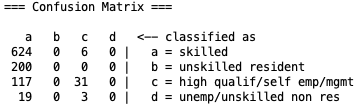
\includegraphics[scale=0.75]{img/conf_matrix.png}
    \caption{J48 Confusion matrix}
    \label{fig:j48_conf_matrix}
\end{figure}

\begin{lstlisting}[caption="J48 rules"\label{fig:j48_rules}]
1. IF credit amount <= 4380 THEN job=skilled
2. IF credit amount > 4380 AND employment=<1 THEN job=skilled
3. IF credit amount > 4380 AND employment=>7 AND purpose=new car THEN job=high qualif/self emp/mgmt
4. IF credit amount > 4380 AND employment=>7 AND purpose=used car THEN job=skilled
5. IF credit amount > 4380 AND employment= 4<=X<7 THEN job=skilled
\end{lstlisting}

Rule 1 states that if someone is asking for a credit amount of less than or equal to 4380 then they have a skilled job, this rule is true for 34.49\% of cases in the dataset. 

Rule 2 shows that if they are asking for a loan larger than 4380 and they have been employed for less than a year they are a in a skilled job. This rule is correct in 35.48\% of cases.

Rule 3 states that if they are asking for a loan greater than 4380, they have been employed for more than 7 years and they are using the loan to buy a new car then they are in a highly qualified/self employed/management job. This is the case for 26.67\% of the occurrences.

Rule 4 shows us that if they are asking for a loan greater than 4380, been employed for more than 7 years and are looking to use the loan to buy a used car they are in a skilled job. This rule is 45\% accurate.

Rule 5 states that if they are asking for a loan greater than 4380, have been employed for between 4 and 7 years then they are in a skilled job. 36.17\% of cases are correctly classified by this rule.

\subsection{Association}

\begin{lstlisting}[caption="Apriori configuration"\label{fig:apriori_config}]
Apriori -N 6 -T 0 -C 0.9 -D 0.05 -U 1.0 -M 0.1 -S -1.0 -c -1
\end{lstlisting}
\begin{lstlisting}[caption="Apriori rules"\label{fig:apriori_rules}]
1. IF checking_status=no checking AND purpose=radio/tv THEN class=good 
    (Confidence = 94%)
2. IF checking_status=no checking AND credit_history=critical/other existing credit THEN class=good 
    (Confidence = 93%)
3. IF checking_status=no checking AND employment=>=7 THEN class=good 
    (Confidence = 93%)
4. IF checking_status=no checking AND personal_status=male single AND job=skilled THEN  class=good 
    (Confidence = 92%)
5. IF checking_status=no checking AND credit_history=existing paid AND job=skilled THEN class=good 
    (Confidence = 90%)

\end{lstlisting}
The Apriori algorithm was run on a nominal version of the dataset. The settings that have been used can be seen in Listing~\ref{fig:apriori_config}. 5 rules were produced that show some interesting patterns in the data these can be seen in Listing~\ref{fig:apriori_rules}. Each rule produces a relatively high confidence level with the lowest being 90\%, this shows that 90\% of the data matches this rule. 

Rule 1 shows us that if a person has no current account with the bank and is applying for a loan for a TV or radio they are considered a good person to lend to, 94\% of the data matches this description.

Rule 2 shows that if even if someone has no current account with the bank they are a good person to lend to even if their credit history is critical or other debts exist at a different bank.

Rule 3 shows that if someone has no current account with the bank but they have been employed for 7 or more years then they are a good person to lend to.

Rule 4 shows that if someone has no current account with the bank but they are a male in a skilled profession then they care a good person to lend money to.

Rule 5 shows that if someone has no current account with the bank but they have paid back all their previous debts on time and have a skilled job the bank can lend them money.

% change confidence
\subsection{Clustering}
SimpleKMeans is a clustering algorithm that was run on the data in order to determine groups of conditions that relate to each other. 6 different clusters were produced by the algorithm with the following settings (Listing~\ref{fig:simplekmeans_config}). Clusters were built on the 'purpose', 'employment', 'age' and 'job' attributes and 5 patterns were drawn from the clusters. These can be seen in the table below.

\begin{lstlisting}[caption="SimpleKMeans configuration"\label{fig:simplekmeans_config}]
SimpleKMeans -init 0 -max-candidates 100 -periodic-pruning 10000 -min-density 2.0 -t1 -1.25 -t2 -1.0 -N 6 -A "weka.core.EuclideanDistance -R first-last" -I 500 -num-slots 1 -S 10
\end{lstlisting}


\begin{table}[h!]
\centering
\label{fig:simplekmeans_rules}
\resizebox{\textwidth}{!}{%
\begin{tabular}{|c|c|}
\hline
Cluster & Overview \\ \hline
1 & \begin{tabular}[c]{@{}c@{}}This is a group of people who have been working in a skilled job between 1-4 years.\\ They are around age 28 and are looking to get a loan for a new car.\end{tabular} \\ \hline
2 & \begin{tabular}[c]{@{}c@{}}This is a group of people who are currently unemployed but they are highly qualified/self employed/management.\\ They are around age 42 and are looking to get a loan for a used car.\end{tabular} \\ \hline
3 & \begin{tabular}[c]{@{}c@{}}This is a group of people who are unskilled residents who have been working for 7 or more years.\\ They are around age 40 and are looking to get a loan for a radio or tv.\end{tabular} \\ \hline
4 & \begin{tabular}[c]{@{}c@{}}This is a group of people who have been working in a skilled job for 7 or more years.\\ They are around age 42 and are looking to get a loan for furniture.\end{tabular} \\ \hline
5 & \begin{tabular}[c]{@{}c@{}}This is a group of people who have been working in a skilled job between 1-4 years.\\ They are around age 32 and are looking to get a loan for a radio.
\end{tabular} \\ \hline
\end{tabular}%
}
\end{table}



\section{Conclusion}
There are many different approaches to analysing data through the use of data mining and machine learning. These approaches come with their own advantages and disadvantage, for instance, clustering can single out interesting points that can help distinguish groups apart from one another. J48, in comparison to clustering, allows a decision tree to be produced and the rules can be presented in a visual format making it easy to see clear patterns. 

From the resulting rules it can be seen that the majority of loans and loan approvals go to people with a skilled job, highly skilled/self employed/management professionals also are often approved. 


\end{document}

